\chapter{Pattern Sequenziali Frequenti}
\label{ch:seq}

Questo capitolo descrive un'analisi effettuata sul solo data set degli studenti. L'idea generale è quella di estrarre dei \textit{pattern sequenziali} dal data set ottenuto nella fase di \textit{preprocessing} descritta in \ref{prepr:seq}, per poi analizzarli ulteriormente con degli script Python realizzati \textit{ad hoc}.

\section{L'algoritmo GSP}

    Per l'estrazione dei pattern sequenziali \textbf{frequenti} è stato fatto uso dell'algoritmo \textit{Generalized Sequential Pattern}. Una breve descrizione del funzionamento di tale algoritmo può essere trovata in \cite{gsp}: \\

    "There are two main steps in the algorithm:
    \begin{itemize}
        \item \textbf{Candidate Generation}. Given the set of frequent (k-1)-frequent sequences F(k-1), the candidates for the next pass are generated by joining F(k-1) with itself. A pruning phase eliminates any sequence, at least one of whose subsequences is not frequent.
        \item \textbf{Support Counting}. Normally, a hash tree–based search is employed for efficient support counting. Finally non-maximal frequent sequences are removed.
    \end{itemize}

    The algorithms for solving sequence mining problems are mostly based on the \textit{a priori} (level-wise) algorithm." \\

    Parafrasando quanto sopra riportato, l'algoritmo GSP è basato sul \textbf{principio Apriori} --- lo stesso già incontrato in \ref{apriori}, per quanto riguardava la ricerca di regole associative. \\

    L'implementazione utilizzata per l'analisi in oggetto, è quella fornita da Weka. Come si può vedere in Figura \ref{gsp_weka}, si tratta di una versione piuttosto basilare in cui si può specificare un limitato numero di parametri; tuttavia, la (poca) flessibilità concessa è risultata sufficiente al raggiungimento dello scopo.

    \begin{figure}
        \centering
        \caption{cose}
        \label{gsp_weka}
        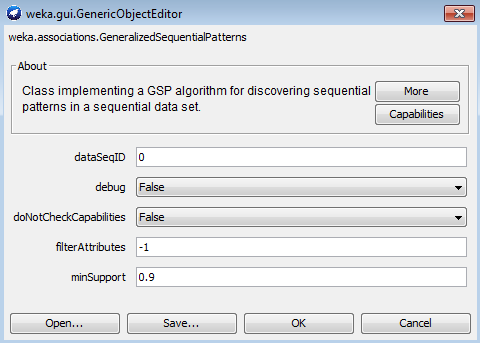
\includegraphics[scale=0.5]{img/gsp.png}
    \end{figure}